\documentclass[12pt,a4paper]{report}

%====En-tête====
% Ajout des packages
\usepackage[english]{babel} % pour dire que le texte est en francais
\usepackage{a4} % pour la taille
\usepackage[T1]{fontenc} % pour les font postscript
\usepackage[cyr]{aeguill} % Police vectorielle TrueType, guillemets francais
\usepackage{epsfig} % pour gérer les images
\usepackage{amsmath,amsthm} % très bon mode mathématique
\usepackage{amsfonts,amssymb,bm, bbold}% permet la definition des ensembles
\usepackage{algorithm2e} % pour les algorithmes
\usepackage{algpseudocode} % pour les algorithmes
\usepackage{float} % pour le placement des figure
\usepackage{url} % pour une gestion efficace des url
\usepackage[colorlinks,citecolor=blueind,urlcolor=blue,bookmarks=false,hypertexnames=true]{hyperref}  % pour les hyperliens dans le document
\usepackage{tocbibind} % Pour avoir des index pour table des matières, biblio
\usepackage{tikz} % For graph plots

%% Bibliography
\usepackage[style=apa,citestyle=authoryear-comp]{biblatex}
\addbibresource{references.bib}


%% Tikz Related
\usetikzlibrary{calc,shapes,backgrounds,arrows,automata,shadows,positioning}
\usetikzlibrary{arrows,shapes,positioning,shadows,trees,calc,backgrounds,automata,positioning}



\tikzset{
    basic/.style  = {draw, text width=3cm, font=\sffamily, rectangle},
    root/.style   = {basic, rounded corners=2pt, thin, align=center,
            fill=green!30},
    level 2/.style = {basic, rounded corners=6pt, thin,align=center, fill=green!60,
            text width=8em},
    level 3/.style = {basic, thin, align=left, fill=pink!60, text width=3.5cm}
}


% pour tickz multilevel
\definecolor{redorg}{RGB}{215,48,39}
\definecolor{orangeorg}{RGB}{253,174,97}

\definecolor{blueind}{RGB}{69,117,233}
\definecolor{cyanind}{RGB}{116,173,209}
\definecolor{electricblue}{RGB}{125, 249, 255}

\definecolor{greenind}{RGB}{112,130,56}

\definecolor{burntorange}{RGB}{204, 85, 0}
\definecolor{goldenyellow}{RGB}{255, 192, 0}
\definecolor{peach}{RGB}{255, 229, 180}

\definecolor{gray}{RGB}{128,128,128}

% Nouvelles commandes
\newcommand{\Tau}{\mathcal{T}}

% titre et auteur
\title{Rapport de stage dans l'UMR MIA Paris-Saclay}
\author{Louis Lacoste}

\begin{document}
\maketitle
\tableofcontents

\chapter{Présentation de l'UMR}

\chapter{Context}

\section{Usage and importance of bipartite graphs}

Bipartite graphs, denoted as $G = (U,V,E)$ with $U$ and $V$ two disjoint and
independent sets of vertices and $E$ the set of edges connecting $U$ vertices to
$V$ vertices.

\begin{minipage}{0.5\linewidth}
    \centering
    Bipartite network\\
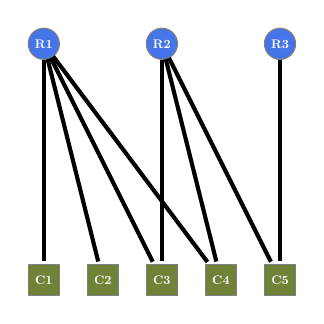
\begin{tikzpicture}[scale=.6]
    \tikzstyle{every edge}=[-,>=stealth',shorten >=1pt,auto,draw,line width=1.5pt]
    \tikzstyle{every state}=[draw, text=white,scale=0.95, transform shape]
    \tikzstyle{every state}=[draw=none,text=white,scale=0.75, transform shape]
    \tikzstyle{every node}=[fill=blueind]

    \node[state, draw=black!50] (A1) at (0,5) {\textbf{R1}};
    \node[state, draw=black!50] (A2) at (2.5,5) {\textbf{R2}};
    \node[state, draw=black!50] (A3) at (5,5) {\textbf{R3}};

    \tikzstyle{every node}=[fill=greenind, shape=rectangle]
    \tikzstyle{every state}=[draw=none,text=white,scale=0.75, transform shape, shape=rectangle]
    \node[state, draw=black!50] (B1) at (0,0) {\textbf{C1}};
    \node[state, draw=black!50] (B2) at (1.25,0) {\textbf{C2}};
    \node[state, draw=black!50] (B3) at (2.5,0) {\textbf{C3}};
    \node[state, draw=black!50] (B4) at (3.75,0) {\textbf{C4}};
    \node[state, draw=black!50] (B5) at (5,0) {\textbf{C5}};
    \path (A1) edge [] (B1);
    \path (A1) edge  (B2);
    \path (A1) edge  (B3);
    \path (A1) edge  (B4);
    \path (A2) edge  (B3);
    \path (A2) edge  (B4);
    \path (A3) edge  (B5);
    \path (A2) edge  (B5);
\end{tikzpicture}
\end{minipage}
\begin{minipage}{0.5\linewidth}
\begin{center}
Incidence matrix
$B=\left(
\begin{array}{rrrrr}
1 &   1 &   1 &   1 &   0 \\ 
    0 &   0 &   1 &   1 &   1 \\ 
    0 &   0 &   0 &   0 &   1 \\  
\end{array}\right)
$\\
\end{center}
\end{minipage}



This representation can be used to represent various forms of interactions were
two kinds of ''actors'' interact. Those interactions can be binary or valued and
a numeric representation is the incidence matrix, in the above example $B$.\\

Among the use case of bipartite graphs one can find the Netflix Problem, which
was a prize organized by Netflix to improve its Recommender system. The row 
nodes are the movies and the columns are the user, at the intersection the value
is the review of the user $j$ for the movie $i$.\\

Another use is the representation of ecological interactions like 
plant-pollinator \parencite{ramos-jilibertoTopologicalChangeAndean2010}, birds-seed
dispersion, prey-predator or
host-parasite \parencite{kaszewska-gilasGlobalStudiesHostParasite2021}.
In those cases, the rows are pollinator species and the columns are plant 
species, and the intersection is a value, binary if it is a presence/absence or
a value if it is an abundance count.

Bipartite graphs are widely used in biology, in various fields, among which the
previously cited ecological networks, but also in medicine with biomedical
networks, biomolecular networks or epidemiological 
networks. \parencite{pavlopoulosBipartiteGraphsSystems2018}


Some interesting results can arise when applying a tool widely used on a particular
kind of interactions is used on another kind of interactions. Companies like
Netflix use recommender system, to recommend another product to consumers based
on their previous interactions.
In \cite{desjardins-proulxEcologicalInteractionsNetflix2017} the authors use the
\emph{K-nearest neighbour} (KNN) algorithm as a Recommender to predict missing
preys for predators in a predator-prey network.

\section{Latent Block Model}

The Latent Block Model (LBM) introduced by \cite{govaertLatentBlockModel2010} 
adapts the Stochastic Block Model (SBM) 
(\cite{hollandStochasticBlockmodelsFirst1983};\cite{snijdersEstimationPredictionStochastic1997})
to bipartite graphs.

\begin{small}
Please note that we prefer the term ''BiSBM'' and will use both LBM and BiSBM to
designate the Stochastic Block model applied on bipartite networks.
\end{small}

This model supposes that:
\begin{itemize}
    \item Row nodes are members of row blocks and column nodes are members of 
    column blocks.
    \item The connectivity of two individuals is determined by their block 
    memberships.
    \item An interaction can only occur between a row and a column node.
\end{itemize}

\begin{figure}[H]
    \center
    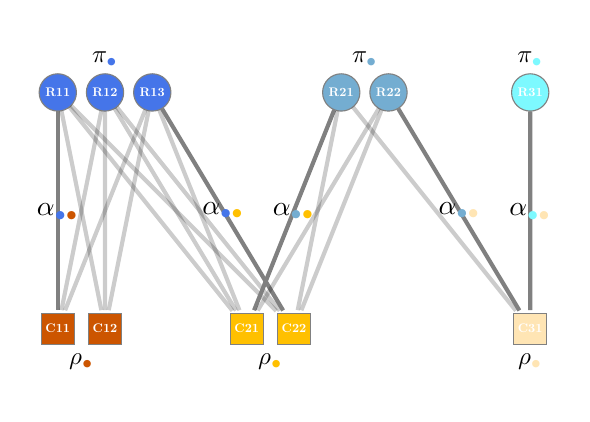
\begin{tikzpicture}[scale=.6]
        \tikzstyle{every state}=[draw, text=white,scale=0.95, transform shape]
        \tikzstyle{every state}=[draw=none,text=white,scale=0.75, transform shape]
        
        \tikzstyle{every node}=[fill=blueind]
        \node[state, draw=white, fill=none, text=black, scale=2] (pi1) at (1,5.7) {\textbf{$\pi_{{\color{blueind}\bullet}}$}};
        \node[state, draw=black!50] (R11) at (0,5) {\textbf{R11}};
        \node[state, draw=black!50] (R12) at (1,5) {\textbf{R12}};
        \node[state, draw=black!50] (R13) at (2,5) {\textbf{R13}};
        
        \tikzstyle{every node}=[fill=cyanind]
        \node[state, draw=white, fill=none, text=black, scale=2] (pi2) at (6.5,5.7) {\textbf{$\pi_{{\color{cyanind}\bullet}}$}};
        \node[state, draw=black!50] (R21) at (6,5) {\textbf{R21}};
        \node[state, draw=black!50] (R22) at (7,5) {\textbf{R22}};
        
        \tikzstyle{every node}=[fill=electricblue]
        \node[state, draw=white, fill=none, text=black, scale=2] (pi3) at (10,5.7) {\textbf{$\pi_{{\color{electricblue}\bullet}}$}};
        \node[state, draw=black!50] (R31) at (10,5) {\textbf{R31}};
    
        \tikzstyle{every node}=[fill=burntorange, shape=rectangle]
        \node[state, draw=white, fill=none, text=black, scale=2] (pi3) at (0.5,-0.7) {\textbf{$\rho_{{\color{burntorange}\bullet}}$}};
        \tikzstyle{every state}=[draw=none,text=white,scale=0.75, transform shape, shape=rectangle]
        \node[state, draw=black!50] (B1) at (0,0) {\textbf{C11}};
        \node[state, draw=black!50] (B2) at (1,0) {\textbf{C12}};
        \tikzstyle{every node}=[fill=goldenyellow, shape=rectangle]
        \node[state, draw=white, fill=none, text=black, scale=2] (pi3) at (4.5,-0.7) {\textbf{$\rho_{{\color{goldenyellow}\bullet}}$}};
        \node[state, draw=black!50] (B3) at (4,0) {\textbf{C21}};
        \node[state, draw=black!50] (B4) at (5,0) {\textbf{C22}};
        \tikzstyle{every node}=[fill=peach, shape=rectangle]
        \node[state, draw=white, fill=none, text=black, scale=2] (pi3) at (10,-0.7) {\textbf{$\rho_{{\color{peach}\bullet}}$}};
        \node[state, draw=black!50] (B5) at (10,0) {\textbf{C31}};

        \tikzstyle{every edge}=[-,>=stealth',shorten >=1pt,auto,draw,line width=1.5pt,draw opacity=0.2]

        \path (R11) edge[-,>=stealth',shorten >=1pt,auto,draw=gray,line width=1.5pt, fill=gray, opacity=1] node[anchor=center, fill=none] {$\alpha_{{\color{blueind}\bullet}{\color{burntorange}\bullet}}$} (B1);
        \path (R11) edge (B2);
        \path (R11) edge  (B3);
        \path (R11) edge  (B4);

        \path (R12) edge [] (B1);
        \path (R12) edge  (B2);
        \path (R12) edge  (B3);
        \path (R12) edge  (B4);

        \path (R13) edge [] (B1);
        \path (R13) edge  (B2);
        \path (R13) edge  (B3);
        \path (R13) edge[-,>=stealth',shorten >=1pt,auto,draw=gray,line width=1.5pt, fill=gray, opacity=1] node[anchor=center, fill=none] {$\alpha_{{\color{blueind}\bullet}{\color{goldenyellow}\bullet}}$} (B4);

        \path (R21) edge[-,>=stealth',shorten >=1pt,auto,draw=gray,line width=1.5pt, fill=gray, opacity=1] node[anchor=center, fill=none] {$\alpha_{{\color{cyanind}\bullet}{\color{goldenyellow}\bullet}}$} (B3);
        \path (R21) edge  (B4);
        \path (R21) edge  (B5);
        
        \path (R22) edge  (B3);
        \path (R22) edge  (B4);
        \path (R22) edge[-,>=stealth',shorten >=1pt,auto,draw=gray,line width=1.5pt, fill=gray, opacity=1] node[anchor=center, fill=none] {$\alpha_{{\color{cyanind}\bullet}{\color{peach}\bullet}}$} (B5);

        \path (R31) edge[-,>=stealth',shorten >=1pt,auto,draw=gray,line width=1.5pt, fill=gray, opacity=1] node[anchor=center, fill=none] {$\alpha_{{\color{electricblue}\bullet}{\color{peach}\bullet}}$} (B5);

    \end{tikzpicture}
\caption{An LBM model visualization}
\label{fig:LBMvisu}
\end{figure}

On \ref{fig:LBMvisu}, $\pi$ are the probabilities for a row node to belong to
the row block of corresponding color, $\rho$ are the probabilities for a column
node to belong to the column block of corresponding color and $\alpha$ are the
connectivity parameters between the row and column blocks.

This model can be used to easily generate bipartite graphs with complex and very
varied structures. But when trying to determine the structure of a given network
we need to find those parameters.

For this a common approach is to use a VEM algorithm
(proposed for SBM in \cite{daudinMixtureModelRandom2008} and for LBM in \cite{govaertEMAlgorithmBlock2005}) 
those groups and the required parameters can be inferred by maximizing a lower
bound of the likelihood minus a penalty.

\section{colSBM model, a joint model for a collection of networks}

The \emph{colSBM} model introduced by \cite{chabert-liddellLearningCommonStructures2023}
propose an extension of the SBM model to collections of SBMs. A collection is a
set of networks which nodes are not common or linked between different networks,
the interactions have the same valuations and are of the same type.

The model can retrieve the shared structure in a collection, indicate
if networks should be grouped in a collection and  in a large pool of networks,
collections with common structures.

The next step after designing this collection model for unipartite was to adapt
it to the bipartite case.

\chapter{Adjustment of colSBM to the bipartite case: colBiSBM}

\section{Definition of the model}
Here are some common notations and conventions that we will use in the following
sections.

\subsection{A collection of i.i.d Bipartite SBM}

As for \emph{colSBM} this first model is the most constrained. It assumes
that all the networks are the independent realizations of the same $Q_1$-$Q_2$-BiSBM
with identical parameters. The \emph{iid-colBiSBM} is defined as follows:

\begin{align}
    \tag{\emph{iid-colBiSBM}}
    X^m \sim \mathcal{F}-BiSBM_{n_1,n_2} (Q_1, Q_2, \bm{\pi}, \bm{\rho}, \bm{\alpha}), \forall m = 1, \dots M,
\end{align}


\section{Variational Expectation step}
Fixed point formula for the Bernoulli distribution:
\begin{itemize}
    \item[-] \textit{iid} :
    \[ \bm{\tau}^{m,1} = ~^{t}\pi + \exp((\text{Mask}^{m} \odot A^{m})
        \bm{\tau}^{m,2} ~^{t}(\text{logit}(\alpha)) + \text{Mask}^{m} 
        \bm{\tau}^{m,2} ~^{t}\log(\bm{1} - \alpha)) \]
    \[ \bm{\tau}^{m,2} = ~^{t}\rho + \exp(~^{t}(\text{Mask}^{m} \odot A^{m}) 
    \bm{\tau}^{m,1} \text{logit}(\alpha) + ~^{t}\text{Mask}^{m} 
        \bm{\tau}^{m,1} \log(\bm{1} - \alpha)) \]
    \item[-] $\rho\pi$ :
        \[ \bm{\tau}^{m,1} = ~^{t}\pi^{m} + \exp((\text{Mask}^{m} \odot A^{m})
            \bm{\tau}^{m,2} ~^{t}(\text{logit}(\alpha)) + \text{Mask}^{m} 
            \bm{\tau}^{m,2} ~^{t}\log(\bm{1} - \alpha)) \]
        \[ \bm{\tau}^{m,2} = ~^{t}\rho^{m} + \exp(~^{t}(\text{Mask}^{m} \odot A^{m}) 
        \bm{\tau}^{m,1} \text{logit}(\alpha) + ~^{t}\text{Mask}^{m} 
            \bm{\tau}^{m,1} \log(\bm{1} - \alpha)) \]
\end{itemize}

with $\text{Mask}^{m}$ the matrix containing $0$ if the value is a NA and a 1
otherwise.

\section{M step of the algorithm}

Incorporate the equations from \parencite{chabert-liddellLearningCommonStructures2023}

\section{Computation of the variational bound}

\section{Penalties}

\paragraph*{\textit{iid-colBiSBM}}
For the \textit{iid-colBiSBM} the penalties were modified in the following way :

\begin{itemize}
    \item For the $\pi$s and $\rho$s:
    \[\text{pen}_{\pi}(Q_1) = (Q_1 - 1)\log(\sum_{m=1}^{M}n_{r}^{(m)})\]
    \[\text{pen}_{\rho}(Q_2) = (Q_2 - 1)\log(\sum_{m=1}^{M}n_{c}^{(m)})\]
    \item For the $\alpha$s :
    \[\text{pen}_{\alpha}(Q_1, Q_2) = Q_1 \times Q_2 \log(N_M)\]
    avec
    \[ N_M = \sum_{m = 1}^{M} n_{r}^{(m)} \times n_{c}^{(m)} \]
\end{itemize}
And thus the $\text{BIC-L}$ formula is now:
\[ \text{BIC-L}(\bm{X},Q_1, Q_2) = \max_{\theta} \mathcal{J} (\mathcal{\hat{R}}, \bm{\theta}) 
- \frac{1}{2} [\text{pen}_{\pi}(Q_1) + \text{pen}_{\rho}(Q_2) + \text{pen}_{\alpha}(Q_1, Q_2)]\]

\paragraph*{\textit{$\rho\pi$-colBiSBM}}
For the \textit{$\rho\pi$-colBiSBM} the penalties are the following:

\begin{itemize}
    \item The support penalties are:
    \[ \text{pen}_{S_1}(Q_1) = -2 \log p_{Q_1} (S_1) \]
    \[ \text{pen}_{S_2}(Q_2) = -2 \log p_{Q_2} (S_2) \]
    with
    \[ \log p_{Q_1}(S_1) = - M \log(Q_1) - \sum_{m=1}^{M} \log {Q_1 \choose Q_1^{(m)}} \]
    \[ \log p_{Q_2}(S_2) = - M \log(Q_2) - \sum_{m=1}^{M} \log {Q_2 \choose Q_2^{(m)}} \]
    \item Penalties for the $\rho$s and $\pi$s:
    \[ \text{pen}_{\pi}(Q_1, S_1) = \sum_{m=1}^{M} (Q_{1}^{(m)} - 1) \log n_{r}^{(m)} \]
    \[ \text{pen}_{\rho}(Q_2, S_2) = \sum_{m=1}^{M} (Q_{2}^{(m)} - 1) \log n_{c}^{(m)} \]
    \item Penalties for the $\alpha$s:
    \[ \text{pen}_{\alpha}(Q_1, Q_2, S_1, S_2) = (\sum_{q=1}^{Q_1} \sum_{r=1}^{Q_2} \mathbb{1}_{(S_1)'S_2 > 0}) \log (N_M) \]
\end{itemize}
And the corresponding BIC-L formula:
\[
    \begin{aligned}
        \text{BIC-L}(\bm{X},Q_1, Q_2) = 
        \max_{S_1,S_2} [
            & \max_{\theta_{S_1,S_2} \in \Theta_{S_1,S_2}} \mathcal{J}(\mathcal{\hat{R}},\theta_{S_1,S_2})\\
            - \frac{1}{2} & (\text{pen}_{\pi}(Q_1, S_1)  + \text{pen}_{\rho}(Q_2, S_2)\\
            &+ \text{pen}_{\alpha}(Q_1, Q_2, S_1, S_2)\\
            &+ \text{pen}_{S_1}(Q_1) + \text{pen}_{S_2}(Q_2))]\\
    \end{aligned}
\]

\section{Latent space exploration and model selection}
In order to explorer the bi-dimensional latent space $(Q_1,Q_2)$
we use the following strategies.

\subsection{Model selection}
In the following steps the model selection consists of using the BIC-L 
criterion to select the model. We choose among the proposed models the one that
maximizes the BIC-L

\subsection{Initialization and pairing of the models}
First to combine the information from the $M$ networks we fit a collection model
for each network at the two points $Q = (1, 2)$ and $Q = (2, 1)$. Using the 
previously described VEM algorithm we obtain for each network its parameters 
($\rho,\pi,\alpha$).

We then compute the marginal laws for each dimension, for each network. Then 
we order the network blocks by the probabilities obtained in decreasing order.
\begin{itemize}
    \item For the memberships on the columns: 
    $col~order_m = order\left(\pi_m \times \alpha_m\right)$ 
    \item For the memberships on the rows:
    $row~order_m = order\left(\rho_m \times ~^{t}(\alpha_m)\right)$ 
\end{itemize}

Using this order we relabel the memberships for the $M$ fitted collection of a
single network.
Then we use the $M$ memberships to fit a collection containing the $M$ networks.
\subsection{Greedy exploration to find an estimation of the mode}
Using the previously fitted models for $Q = (1,2)$ and $Q = (2,1)$ we choose to
perform a greedy exploration to find a first mode.

Meaning that for a given $Q = (Q_1, Q_2)$ we will compute all the possible 
memberships for the points $Q \in \{(Q_1 + 1, Q_2),(Q_1, Q_2 + 1),(Q_1 - 1, Q_2),
(Q_1, Q_2 - 1)\}$, fit
the corresponding models and choose the one that maximizes the BIC-L as the 
next point from which to repeat the procedure. We repeat the procedure until the
BIC-L stops increasing $2$ times in a row.

\begin{algorithm}[H]
    \caption{Greedy Exploration for Mode Estimation}
    \SetAlgoLined
    \SetKwInOut{Input}{Input}
    \SetKwInOut{Output}{Output}
    
    \Input{Fitted models for $Q = (1,2)$ and $Q = (2,1)$}
    \Output{Estimation of the mode using greedy exploration}
    
    \BlankLine
    Initialize $Q = (1,2)$ as the starting point
    Initialize $\text{BIC-L}_{\text{max}}$ as the maximum achieved BIC-L value
    Initialize $consecutive\_count$ as 0
    
    \BlankLine
    \While{$consecutive\_count < 2$}{
        Compute possible memberships for $Q \in \{(Q_1 + 1, Q_2), (Q_1, Q_2 + 1), (Q_1 - 1, Q_2), (Q_1, Q_2 - 1)\}$\;
        Fit models with the computed memberships
        Choose the model with the maximum BIC-L as the next point
        
        \BlankLine
        \If{$\text{BIC-L} > \text{BIC-L}_{\text{max}}$}{
            $\text{BIC-L}_{\text{max}} \leftarrow \text{BIC-L}$
            $consecutive\_count \leftarrow 0$
        }
        \Else{
            $consecutive\_count \leftarrow consecutive\_count + 1$
        }
        
        \BlankLine
        $Q \leftarrow$ Next selected point
    }
    
    \BlankLine
    \textbf{Output:} Estimation of the mode using greedy exploration
\end{algorithm}

When this first estimation of the BIC-L mode has been find we apply the moving
window on it.
\subsection{Moving window to update the block memberships and the BIC-L}
The \emph{moving window} is used to update the block memberships on rows and 
columns and fit new models with those changes.
To define the window, we use a center point and a \emph{depth}, giving us the 
bottom left corner ($Q_{1,center} - depth, Q_{2,center} - depth$) and the top right corner of the 
window ($Q_{1,center} + depth, Q_{2,center} + depth$). All the points in this square will be 
updated and contribute to the update of the others.
This procedure is repeated until convergence of the BIC-L.

The procedure consists of two alternating steps:
\begin{itemize}
    \item the \emph{forward pass}: repeatedly computing the possible splits to 
    fit the current model.
    \item the \emph{backward pass}: computing the possible merges to fit the current model.
\end{itemize}


\begin{algorithm}[H]
    \caption{Moving Window Procedure}
    \SetAlgoLined
    \SetKwInOut{Input}{Input}
    \SetKwInOut{Output}{Output}

    \Input{Center point $(Q_{1,\text{center}}, Q_{2,\text{center}})$, depth}
    \Output{Best model with maximum BIC-L in the window}

    \BlankLine
    Define bottom left corner $(Q_{1,\text{center}} - \text{depth}, Q_{2,\text{center}} - \text{depth})$\\
    Define top right corner $(Q_{1,\text{center}} + \text{depth}, Q_{2,\text{center}} + \text{depth})$

    \BlankLine
    \While{not converged}{
        \textbf{Forward pass:}

        \For{$Q_1 \in \left[ Q_{1,\text{center}} - \text{depth} ; Q_{1,\text{center}} + \text{depth} \right]$}{
            \For{$Q_2 \in \left[ Q_{2,\text{center}} - \text{depth}; Q_{2,\text{center}} + \text{depth} \right] $}{
                Compute possible splits from predecessors $(Q_1 - 1, Q_2)$ and $(Q_1, Q_2 - 1)$
                Fit models with the block membership changes
                Compare and keep the best model based on BIC-L
            }
        }

        \BlankLine
        \textbf{Backward pass:}

        \For{$Q_1 \in \left[ Q_{1,\text{center}} + \text{depth} ; Q_{1,\text{center}} - \text{depth} \right]$}{
            \For{$Q_2 \in \left[ Q_{2,\text{center}} + \text{depth}; Q_{2,\text{center}} - \text{depth} \right] $}{
                Compute possible merges from predecessors $(Q_1 + 1, Q_2)$ and $(Q_1, Q_2 + 1)$
                Fit models with the block membership changes
                Compare and keep the best model based on BIC-L
            }
        }

        \BlankLine
        Update the best model based on the maximum BIC-L
    }

    \BlankLine
    \textbf{Output:} Best model with maximum BIC-L in the window
\end{algorithm}


\paragraph*{Forward pass} The forward pass consists for a model at $(Q_1, Q_2)$ 
to compute the possible splits from the block memberships of its "predecessors". 
The predecessors are the point at the left $(Q_1 - 1, Q_2)$ and below 
$(Q_1, Q_2 - 1)$ the current model (if they exist). To update the current model,
we take its predecessors block memberships and try to split one of the blocks in
two. Then the current model is fitted using this clustering as a starting 
clustering. Once all the possible splits are fitted, they are compared, keeping 
the best, in the sense of the BIC-L. If a model was already present it is also
compared and the best is chosen as the model for this round at $(Q_1, Q_2)$.\\
The procedure then repeats for the point at $(Q_1 + 1, Q_2)$ until it reaches 
$(Q_{1,center} + depth, Q_2)$ from which it repeats from 
$(Q_{1,center} - depth, Q_2 + 1)$. This repeats until computing the best model
for $(Q_{1,center} + depth, Q_{2,center} + depth)$.
\textit{Note on the initialization:} The forward pass starts from the point 
$(Q_{1,center} + depth, Q_{2,center} + depth)$, so this points needs to have at 
least a model fitted. In the best case, the greedy exploration will have visited
this point. But if the point has not been visited, a model will be fitted from
a spectral initialization (i.e the block memberships is computed by using a 
spectral clustering). From this point, the next model will have at least one
predecessor and the procedure can iterate.

\paragraph*{Backward pass} The backward pass consists for a model at $(Q_1, Q_2)$ 
to compute the possible merges from the block memberships of its "predecessors". 
The predecessors are the point at the right $(Q_1 + 1, Q_2)$ and on top 
$(Q_1, Q_2 + 1)$ of the current model (if the predecessors exist). To update the
current model, we take its predecessors block memberships and try to merge two 
blocks in one. Then the current model is fitted using this clustering as
a starting clustering. Once all the possible merges are fitted, they are
compared, keeping the best, in the sense of the BIC-L.
If a model was already present it is also
compared and the best is chosen as the model for this round at $(Q_1, Q_2)$.\\
The procedure then repeats for the point at $(Q_1 - 1, Q_2)$ until it reaches 
$(Q_{1,center} - depth, Q_2)$ from which it repeats from 
$(Q_{1,center} - depth, Q_2 - 1)$. This repeats until computing the best model
for ($Q_{1,center} - depth, Q_{2,center} - depth$).
\textit{Note on the initialization:} The backward pass starts from
$(Q_{1,center} + depth, Q_{2,center} + depth)$, we know it was initialized at
least by the forward pass, no special case here.\\

At the end of the moving window pass, the model of max BIC-L is the new best
fit and the procedure can repeat until convergence.

\section{Networks clustering}
As in \parencite{chabert-liddellLearningCommonStructures2023} we use a recursive
algorithm to determine the best clustering of the given networks. The procedure
being the same, only the technical modifications for the bipartite case will be
explained below.
\subsection{Distance between two networks}
The distance weights uses $\pi$ and $\rho$.
\[ 
    D_{\mathcal{M}}(m,m') = \sum_{q = 1}^{Q_1} \sum_{r = 1}^{Q_2} \max(\widetilde{\pi}_{q}^{m}, \widetilde{\pi}_{q}^{m'}) \left( \frac{\widetilde{\alpha}_{qr}^{m}}{\widehat{\delta}_{m}} - \frac{\widetilde{\alpha}_{qr}^{m'}}{\widehat{\delta}_{m'}}\right)^{2} \max(\widetilde{\rho}_{r}^{m}, \widetilde{\rho}_{r}^{m'}) 
\]


\printbibliography
\listoffigures
\listoftables
\end{document}